\pagebreak

\section{FPGA to CPU interface Library File - xilinx/cpu.3pl}
\label{chap:lmxilcpulib}

    \index{library!xilinx/cpu.3pl}
    This library provides a class for basic FPGA-CPU interface for platforms
    which provide a communications path between a CPU and FPGA. This includes
    the zynq FPGA and various FPGA prototype boards which have a USB port for
    configuration loading and serial data communications. These procedures allow
    the CPU to read and write static variables, queues and memories and the FPGA
    to interrupt the CPU.
    
    This library contains alternative interfaces for reading and writing 3PL
    variables from the CPU. There are class procedures which are mode-specific - \\
            \hspace*{1cm}{\bf CPU\_API.read\_value()}\\
            \hspace*{1cm}{\bf CPU\_API.read\_queue()}\\
            \hspace*{1cm}{\bf CPU\_API.read\_memory()}\\
            \hspace*{1cm}{\bf CPU\_API.write\_static()}\\
            \hspace*{1cm}{\bf CPU\_API.write\_queue()}\\
            \hspace*{1cm}{\bf CPU\_API.write\_memory()}\\
    and there are generic class procedures - \\
            \hspace*{1cm}{\bf CPU\_API.read()}  \\          
            \hspace*{1cm}{\bf CPU\_API.write()}\\
    
    The former have the advantage that the mode of the variable being accessed
    is reflected in the procedure identifer and this may improve the readability
    the source code. On the other hand the latter are generic and shorter.
    
    There are DMA class modules for reading and writing CPU memory from the
    FPGA -\\
            \hspace*{1cm}{\bf CPU\_API.dma\_read()} \\
            \hspace*{1cm}{\bf CPU\_API.dma\_write()}\\
    and an interrupt class module and an interrupt class procedure -\\
            \hspace*{1cm}{\bf CPU\_API.sigint()}\\
            \hspace*{1cm}{\bf CPU\_API.interrupt()}\\
            
    For example the following three examples are equivalent - 

    \begin{lstlisting}[gobble=12, language=threepl]
        cpu_api.read_queue(entries, , acc <- q, "QR", true, 10 );
    \end{lstlisting}

    \begin{lstlisting}[gobble=12, language=threepl]
        cpu_api.read_queue(entries, , acc <- q, "QR", wordcount=true, ilevel=10 );
    \end{lstlisting}

    \begin{lstlisting}[gobble=12, language=threepl]
        cpu_api.read(count=entries, access=acc <- q, "QR", wordcount=true, ilevel=10);
    \end{lstlisting}
    
    A more detailed description of use of this class can be found in
    (\autorefph{ch:serialcpu}) for platforms with a USB serial link to the
    FPGA and (\autorefph{ch:zynqcpu}) for Zynq platforms. These sections
    include both C and Python3 coding examples.
    
    
    This library is incorporated by using a {\bf source} statement -
    \begin{lstlisting}[gobble=4, language=threepl]
       source "xilinx/cpu.3pl"
    \end{lstlisting}
    {\bf however this library is already included via xilinx/uart\_cpu.3pl
    (\autorefph{chap:lmuartcpulib}) or xilinx/zynq\_axi.3pl
    (\autorefph{chap:lmzynqaxilib}) and so should not be included directly by
    application programs.}

    
    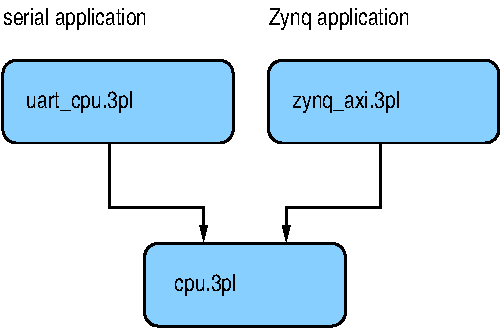
\includegraphics{cpu}

    
    xilinx/zynq\_axi.3pl is included in -\\
    boards/avnet/microzed\_7010.3pl\\
    boards/avnet/microzed\_7020.3pl\\
    boards/digilent/zybo.3pl
    
    xilinx/uart\_cpu.3pl is included in -\\
    boards/avnet/aes\_sp3a\_eval400.3pl\\
    board/gadget\_factory/papilio\_one\_100.3pl\\
    board/gadget\_factory/papilio\_one\_250.3pl\\
    board/gadget\_factory/papilio\_one\_500.3pl\\
    board/gadget\_factory/papilio\_pro\_lx4.3pl\\
    board/gadget\_factory/papilio\_pro\_lx9.3pl
    
    The class for the FPGA interface is created by -
    
    \begin{lstlisting}[gobble=4, language=threepl]
    class(cpu, CPU_API());
    \end{lstlisting}

    cpu.3pl -
    \blist   
    \item   defines class {\bf busCommon} which is used to describe each
            interface.    
    \item   creates an instance of class {\bf CPU\_CODEGEN} whose procedures
            create the logic to implement each type of interface.        
    \item   creates an instance of class {\bf CPU\_API} whose modules
            provide the application program interface. Procedures within
            this class create instances of {\bf busCommon} and add them to
            an interface list. {\bf busCommon} contains all the information
            necessary to create a CPU interface. Class {\bf CPU\_API} in
            turn assigns module create\_bus\_interfaces() as a trailer
            module.
    \blend
    
    Module create\_bus\_interfaces() executes at the end of immediate execution
    (it is a trailer module). It creates the basic CPU interface logic by
    calling module {\bf cpu\_interface} and then traverses the interface list
    and creates code for each interface via procedures in class {\bf
    CPU\_CODEGEN}.
    
    {\bf CPU\_API}, {\bf CPU\_CODEGEN}, {\bf create\_bus\_interfaces} and
    {\bf cpu\_interface} are defined in both UART\_CPU.3pl and zynq\_axi.3pl,
    as the underlying interface logic is quite different for the two platforms.






    \subsection{class library modules}
            
                
        \subsubsection{CPU\_API.signal\_interrupt - interrupt from a signal}\label{sec:lpcpusigint}

            {\bf Library: xilinx/cpu.3pl}

            {\bf Prototype:} \\
            \vsp
            \begin{lstlisting}[gobble=12, language=threepl]

                module
                signal_interrupt (str(event), value(sig, "log")) {}
            \end{lstlisting}

            {\bf Output parameters:} \\
            
            none.

            {\bf Input parameters:} \\
            {\bf event} is the event identifier string.\\
            {\bf sig} is the signal causing the event.\\
        
            {\bf In-line target execution:} \\
            no

            {\bf description:} \\
            This procedure generates a module which will cause a CPU interrupt
            when its input signal {\bf sig} is asserted.
            The argument to parameter {\bf event} is an identifier with
            which to refer to the interrupt in the CPU interface software.

            See also class procedure {\bf interrupt()}
            \autorefph{sec:lpcpuint} which generates a CPU interrupt when
            executed in the FPGA.
    
     
     
     
     
        \subsubsection{CPU\_API.dma\_read - DMA transfer to FPGA from CPU}\label{sec:lpcpudmar}

            {\bf Library: xilinx/cpu.3pl}

            {\bf Prototype:} \\
            \vsp
            \begin{lstlisting}[gobble=12, language=threepl]
                module
                dma_read (
                    queue(data, "bits:64")      // read data
                    <-
                    queue(address, "uint:32"),  // memory address
                    queue(burstlen, "uint:4"),  // burst length - 1
                    int(bus)                    // HP bus 0 to 3
                ) {}
            \end{lstlisting}

            {\bf Output parameters:} \\
            
            {\bf data} is the queue to which data from the transfer is returned.\\

            {\bf Input parameters:} \\
            {\bf address} is a queue supplying the CPU memory physical read address.\\
            {\bf burstlen} is a queue giving the burst length in the case of Zynq.\\
            {\bf bus} is the HP bus, 0 to 3, in the case of Zynq.\\
        
            {\bf In-line target execution:} \\
            no

            {\bf description:} \\
            This procedure generates a module which reads data from the CPU
            memory. For platforms with serial communications between the
            FPGA and the CPU this is not really DMA but instead data is transferred
            from CPU memory by a software thread.
            
            In the case of a platform with a serial interface only one input
            argument, {\bf address}, is valid - {\bf burstlen} and {\bf bus} must
            not be given arguments. \bf{This address is relative to a base address
            set by calling} {\bf set\_dma\_address()} \autorefph{tools_c_serial}.
            
            When an address becomes available on the {\bf address} input queue
            and the output {\bf data} queue is not full a DMA transfer (read)
            will take place. For a serial interface platform this is not a real
            DMA transfer but is carried out in software by a separate CPU
            thread.

            For the Zynq the address is a physical address. When an address and
            a burstlength become available on the {\bf address} and {\bf
            burstlen} input queues and the output {\bf data} queue is not full,
            a DMA transfer (read) will take place. The HP bus selected cannot be
            used for any other interfaces.

            See also class module {\bf CPU\_API.dma\_write()}
            \autorefph{sec:lpcpudmaw} which generates a DMA write module.



        \subsubsection{CPU\_API.dma\_write - DMA transfer from FPGA to CPU}\label{sec:lpcpudmaw}

            {\bf Library: xilinx/cpu.3pl}

            {\bf Prototype:} \\
            \vsp
            \begin{lstlisting}[gobble=12, language=threepl]
                module
                dma_write (
                    queue(data, "bits:64"),     // write data
                    queue(address, "uint:32"),  // memory address
                    queue(burstlen, "uint:4"),  // burst length - 1
                    int(bus)                    // HP bus 0 to 3
                ) {}
            \end{lstlisting}

            {\bf Output parameters:} \\
            
            None.

            {\bf Input parameters:} \\
            {\bf data} is a queue supplying data for the transfer.\\
            {\bf address} is a queue supplying the CPU memory physical write address.\\
            {\bf burstlen} is a queue giving the burst length in the case of Zynq.\\
            {\bf bus} is the HP bus, 0 to 3, in the case of Zynq.\\
        
            {\bf In-line target execution:} \\
            no

            {\bf description:} \\
            This procedure generates a module which writes data to the CPU
            memory. For platforms with serial communications between the
            FPGA and the CPU this is not really DMA but instead data is transferred
            to CPU memory by a software thread.
            
            In the case of a platform with a serial interface only two input
            arguments, {\bf data} and {\bf address}, are valid - {\bf burstlen}
            and {\bf bus} must not be given arguments. \bf{This address is
            relative to a base address set by calling} {\bf set\_dma\_address()}
            \autorefph{tools_c_serial}.
            
            When data and an address become available on the {\bf data} and {\bf
            address} input queues a DMA transfer (read) will take place. For a
            serial interface platform this is not a real DMA transfer but is
            carried out in software by a separate CPU thread.

            For the Zynq When data, an address and a burstlength become available
            on the {\bf data}, {\bf address} and {\bf burstlen} input queues a
            DMA transfer (write) will take place. The HP bus selected cannot be
            used for any other interfaces.

            See also class module {\bf CPU\_API.dma\_read()}
            \autorefph{sec:lpcpudmar} which generates a DMA read module.



    
    \subsection{class library procedures}
            
                
        \subsubsection{CPU\_API.interrupt - interrupt procedure}\label{sec:lpcpuint}

            {\bf Library: xilinx/cpu.3pl}

            {\bf Prototype:} \\
            \vsp
            \begin{lstlisting}[gobble=12, language=threepl]

                procedure
                interrupt (str(event)) {}
            \end{lstlisting}

            {\bf Output parameters:} \\
            
            none.

            {\bf Input parameters:} \\
            {\bf event} is the event identifier string.\\
        
            {\bf In-line target execution:} \\
            yes

            {\bf description:} \\
            This procedure generates an interrupt when executed in the FPGA.
            The argument to parameter {\bf event} is an identifier with
            which to refer to the interrupt in the CPU interface software.

            See also class module {\bf signal\_interrupt()}
            \autorefph{sec:lpcpusigint} which creates a module which sources an
            interrupt from a signal.





        \subsubsection{CPU\_API.read - a CPU-readable interface}\label{sec:lpcpuread}

            {\bf Library: xilinx/cpu.3pl}

            {\bf Prototype:} \\
            \vsp
            \begin{lstlisting}[gobble=12, language=threepl]
                procedure
                read (
                        static(access, "log"),
                        varargs
                        <- 
                        str(name),
                        var(in),
                        varargs
                    ) {}
            \end{lstlisting}

            {\bf Output parameters:} \\
            {\bf access} is an optional static logical variable which is true
            for one clock cycle following a CPU read.
            {\bf varargs} optional output, parameters {\bf out} and {\bf count}.\\

            {\bf Input parameters:} \\
            {\bf in} is the value, queue, cmemory or rmemory mode variable
            to be read.\\
            {\bf name} is a string identifier for the interface.\\
            {\bf varargs} optional input parameters {\bf wordcount}, {\bf ilevel} and
                {\bf port}.\\
        
            {\bf In-line target execution:} \\
            no

            {\bf description:} \\
            This procedure creates a module which provides a CPU-readable
            interface for the the CPU for  3PL variables of mode value, static,
            queue, cmemory or rmemory.
            
            In the case of Zynq the interface uses AXI bus GP0.            
            The size of the input data type must not exceed 256 bits as the CPU
            interface software limits burst transfers to 8 32-bit words.
            
            Boards having a serial interface to the CPU use that interface.
            The size of the input data type must not exceed 1016 bits (127 bytes).
            
            The module is created at the end of immediate execution from
            arguments queued by this procedure. It can be any type, primitive or
            compound.
                        
            It is a common wrapper for the procedures \\
            {\bf CPU\_API.read\_value()} \autorefph{sec:lpcpurdvalue} \\
            {\bf CPU\_API.read\_queue()} \autorefph{sec:lpcpurdqueue} \\
            {\bf CPU\_API.read\_memory()} \autorefph{sec:lpcpurdmem} \\
            
            Parameter {\bf name} is a string identifier that can be used
            in the CPU code to refer to this interface.
            
            Parameter {\bf in} is the input variable or expression to be read
            by the CPU.
           
            Optional input and output varargs parameters are -
            
            \begin{tabular}{| l | l | l |}
            \hline
                    & input varargs         & output varargs    \\
            \hline \hline
            value   &                       &                   \\
            static  &                       &                   \\
            \hline
            queue   &   wordcount ilevel    & out count         \\
            \hline
            cmemory & port                  &                   \\
            rmemory &                       &                   \\
            \hline
            \end{tabular}




            
            \vspace{\baselineskip}\vspace{\baselineskip}
            {\Large \bfseries Value or Static mode}

                
                            Parameter {\bf in} is the value-mode input variable or expression.
            Since it is value mode the argument may be a value mode variable,
            static mode variable or an expression containing these. An expression
            must not contain a queue read.            
            
            The module is created at the end of immediate execution from arguments
            queued by this procedure. It can be any type, primitive or compound. The
            optional output static logical variable {\bf access} goes true for one
            clock cycle to indicate that a read has occurred.
            
            This procedure can be called via the more cryptic and general
            procedure {\bf cpu\_api.read()} \autorefph{sec:lpcpuread} instead.
            
            In the case of Zynq the interface uses AXI bus GP0.            
            The size of the input data type must not exceed 256 bits as the CPU
            interface software limits burst transfers to 8 32-bit words.
            
            Boards having a serial interface to the CPU use that interface.
            The size of the input data type must not exceed 1016 bits (127 bytes).
            

            The optional output static logical variable {\bf access} goes true
            for one clock cycle to indicate that a read has occurred.
            
            The clock domain of output {\bf access} need not be the same as
            that of {\bf in}. If {\bf access} has no clock domain it will be
            given the bus clock domain.
            
            The parameters associated with this bus interface, including an
            allocated bus address, are written
            to the {\em design}.info file.

            The utility info2c is used to process this file and create
            an include file {\em design}.h which contains a funcion
            definition to access this interface. for example the 3PL
            code
            \begin{lstlisting}[gobble=12, language=threepl]
               cpu_read_value("alpha", v);
            \end{lstlisting}
            will result in info2c producing a declaration like
            \begin{lstlisting}[gobble=12, language=C]
               uint32_t alpha_read (fpga_t * fpga) {}
            \end{lstlisting}
            
            When the CPU reads a value it is sampling that value, hence data may
            be lost if the sampling rate is lower than the rate at which data
            changes. The data sampling logic ensures that the data is a valid
            sample even when the source is changing at the time of the
            read. This is a primitive interface which depends on additional
            protocols being imposed by the application code. For example to
            guarantee data integrity a write to register the data in a static
            variable prior to reading could be used. For a more complex interface see {\bf cpu\_api.read\_queue()}
            \autorefph{sec:lpcpurdqueue}.
            
            On running info2c on the .json file the following C function will have been
            defined for interface {\em name} -
            
            \begin{tabular}{| l | l |}
            \hline
            function                   &                 \\ \hline \hline
            fpga\_{\em name}\_read()   & read a datum    \\ \hline
            \end{tabular}
            
            Example: \\
            If 3PL source file prog.3pl contains the following \\
            \begin{lstlisting}[gobble=12, language=threepl]
               class(cpu, cpu_api());
               
               static(s, "uint:16");
               .
               .
               cpu.read_value("S1", s);
               .
               .
            \end{lstlisting}
            the CPU code should contain something like \\
            \begin{lstlisting}[gobble=12, language=C]
                   #include "prog_fpga.h"
                   .
                   .
                   fpga_t *fpga = NULL;
                   int     d;
                   .
                   .
                   fpga_open(portName);
                   .
                   .
                   d = fpga_S1_read(fpga);
                   .
            \end{lstlisting}
            
            This procedure creates no in-line target code so the current clock domain
            when this procedure is called is not relevant. The clock domain is not
            changed by this procedure,
            The CPU code in Python3 should contain something like \\
            \begin{lstlisting}[gobble=12, language=python]
                import sys
                sys.path.append("/Users/......./install/3pl")
                import info2py
                import prog_fpga as fpga

                fpga_open()

                fpga = info2py.info_from_file("prog")   # load info from prog.info file

                d = fpga.P1_read()

            \end{lstlisting}

                        


            \vspace{\baselineskip}\vspace{\baselineskip}
            {\Large \bfseries Queue mode}
                        


                            Parameter {\bf in} is the queue-mode input variable.
            
            The queue must be written somewhere in the program (queues without
            sources result in a fatal error on completion of immediate
            execution). When the module is created the argument queue must have
            an established write clock domain or a fatal error is generated.

            If the input queue is read anywhere else in the program (i.e. other
            than in this module) then it must be read in the bus clock domain
            since that is the clock domain in which it is read in the module
            created by this procedure.

            If optional parameter {\bf wordcount} has an argument and it
            is true, the number of words in the queue buffer can be interrogated
            by the CPU. The input queue may have any of the allowed buffer sizes.
            If the queue is asynchronous, i.e. the read domain is not the bus
            clock domain, the count will not be exact but will be a guaranteed
            minimum number of readable data.

            If optional parameter {\bf wordcount} has an argument and it
            is false, the data returned from reading the number of words in the
            buffer is 0 or 1 instead of a count. A return of 1 means the queue
            buffer is not empty, i.e. can be read. This option is provided to
            simplify the logic where a simple empty/non-empty status is required.

            If optional parameter {\bf wordcount} has no argument then
            there will no interface to directly read the number of words in the
            queue buffer, however an interrupt may be used instead.            

            Note that an empty queue is guaranteed to return all ones to the CPU
            when read. For most data types this single value will usually be
            invalid and hence in that case it can be used as an indication of an
            empty queue. This can be used instead of explicitly reading the
            available word count.

            If an argument to optional parameter {\bf ilevel} is provided then a
            level interrupt on queue buffer status is established as follows -

            If there is no argument then no interrupt is provided.

            If the argument is type "log" with value false then the interrupt will
            be asserted when the queue buffer is not empty.

            If the argument is type "log" with value true then the interrupt will be
            asserted when the number of words in the buffer equals or exceeds a
            level which has been written to the interface from the CPU. The initial
            value of this level is 1. A level value of 0 should not be written to
            the interface as that will result in a continuous level interrupt
            regardless of queue state.

            If the argument is type "uint" or "int" then the interrupt will be
            asserted when the number of words in the buffer equals or exceeds the
            fixed value specified by the integer argument.

            The optional output parameter {\bf count} provides a count of the
            number of data in the queue. The inbuilt function queuewords() can
            only be used in a module which reads the queue, which is usually not
            the case where {\bf cpu\_api.read\_queue()} is the queue destination.
            {\bf count} must have clock domain {\bf bus\_clk}. If it has no clock
            domain, {\bf cpu\_api.read\_queue()} will set it to {\bf bus\_clk}.
            The width of {\bf count} must be sufficient to hold the input queue
            depth.

            If optional output parameter {\bf out} has an argument, each datum
            read from the input queue {\bf in} to the CPU local bus is also
            written to queue {\bf out}. The type of {\bf out} must be such that
            it can be assigned from {\bf in}. {\bf out} should not be allowed to
            block since it cannot stop data being popped from {\bf in} to the CPU
            bus. While {\bf out} in unavailable for writing, no attempt is made
            to write data popped from {\bf in} to it.

            If optional output parameter {\bf access} has an argument, the static
            variable of type "log" is assigned true for one clock cycle every
            time a datum is popped from the input queue {\bf in}. {\bf access}
            may have any clock domain.
            
            On running info2c on the .json file the following C functions will have
            been defined for interface {\em name} -
            
            \begin{tabular}{| l | l | l |}
            \hline
            function                                 & action when?           &                         \\ \hline \hline
            fpga\_{\em name}\_read()                 & always                 & read a datum            \\ \hline
            fpga\_{\em name}\_avail\_read()          & wordcount has argument & read number of words    \\ \hline
            fpga\_{\em name}\_avail\_thresh\_write() & ilevel "log" true      & set interrupt threshold \\ \hline
            fpga\_{\em name}\_enable()               & ilevel has argument    & enable interrupt        \\ \hline
            fpga\_{\em name}\_disable()              & ilevel has argument    & disable interrupt       \\ \hline 
            fpga\_{\em name}\_wait()                 & ilevel has argument    & wait on interrupt       \\ \hline  
            \end{tabular}
            
            Example: \\
            If 3PL source file prog.3pl contains the following \\
            \begin{lstlisting}[gobble=12, language=threepl]
                class(cpu, cpu_api());
                
                queue(p, "uint:16");
                .
                .
                cpu.read("P1", p, wordcount=false, ilevel=false);
                .
                .
            \end{lstlisting}
            the CPU code in C should contain something like \\
            \begin{lstlisting}[gobble=12, language=C]
                #include "prog_fpga.h"
                .
                .
                fpga_t *fpga = NULL;
                int     d[...];
                int     i = 0;
                .
                .
                fpga_open();
                .
                .
                fpga_P1_event_wait(fpga);
                while (fpga_P1_avail_read(fpga) != 0)
                    d[i++] = fpga_P1_read(fpga);
                .
            \end{lstlisting}
            The code will wait until the queue p goes from empty to non-empty
            when an interrupt will release the wait. A loop while the queue
            remains non-empty reads until the queue is empty. Note that since
            {\bf wordcount} is given an argument but the value is false, the count
            will only have values 0/1 for empty/not-empty.
           
            This procedure creates no in-line target code so the current clock
            domain when this procedure is called is not relevant. The clock domain
            is not changed by this procedure,
            
            The CPU code in Python3 should contain something like \\
            \begin{lstlisting}[gobble=12, language=python]
                import sys
                sys.path.append("/Users/......./install/3pl")
                import info2py
                from cpu_serial import *

                fpga_open()

                fpga = info2py.info_from_file("prog")   # load info from prog.info file

                d = []
                fpga.P1_wait()
                while (fpga.P1_avail_read() != 0)
                    d.append = fpga.P1_read()

            \end{lstlisting}
            
            Note that in the unusual case where a queue variable is both read and
            written by the CPU and is not otherwise accessed in the FPGA the input
            and output clock domains of the queue will be undefined. To overcome
            this the clock domain can be set when the queu is created, e.g.
            
            \begin{lstlisting}[gobble=12, language=threepl]
            queue(q, "uint10", domain=null);
            \end{lstlisting}
            
            which will set both the input (write) and output (read) clock domains
            to the current clock domain - see \autorefph{sec:ipqueue}).

                        


            
            \vspace{\baselineskip}\vspace{\baselineskip}
            {\Large \bfseries cmemory or rmemory mode}
            
                        
                            Parameter {\bf in} is the cmemory-mode or rmemory-mode input variable.
            
            If optional output parameter {\bf access} has an argument, the
            static variable of type "log" is assigned true for one clock cycle
            every time the port of {\bf in} is read. {\bf access} may have any
            clock domain.
            
            In the case of Zynq the interface uses AXI bus GP0.            
            The size of the input data type must not exceed 256 bits as the CPU
            interface software limits burst transfers to 8 32-bit words.
            
            Boards having a serial interface to the CPU use that interface.
            The size of the input data type must not exceed 1016 bits (127 bytes).
            
            This interface can use any memory port and that port can also be
            used by other application code, but no arbitration of shared access
            via a port is provided. Coincident access will usually result in
            data corruption. If it is not feasible to dedicate a port to CPU
            access then the CPU application code must limit acccess to the
            memory to times when it is known that the FPGA logic will not also
            be accessing the memory port.
            
            On running info2c on the .json file the following C function will have been
            defined for interface {\em name} -
            
            \begin{tabular}{| l | l |}
            \hline
            function                 &                                \\ \hline \hline
            fpga\_{\em name}\_read() & read a datum from FPGA memory  \\ \hline
            \end{tabular}
            
            Example: \\
            If 3PL source file prog.3pl contains the following \\
            \begin{lstlisting}[gobble=12, language=threepl]
               class(cpu, cpu_api());
               rmemory(m, 2, "uint:8", "uint:16");
               .
               .
               cpu.read_memory("MEM1", m, 0);
               .
               .
            \end{lstlisting}
            then for zynq the CPU code should contain something like \\
            \begin{lstlisting}[gobble=12, language=C]
                   #include "prog.h"
                   .
                   .
                   fpga_t *fpga = NULL;
                   int     d;
                   .
                   .
                   fpga_open();
                   .
                   .
                   d = fpga_MEM1_read(addr);
                   .
            \end{lstlisting}
            where addr is the memory address. The returned data is assigned
            to variable {\bf d}.

            This procedure creates no in-line target code so the current clock domain
            when this procedure is called is not relevant. The clock domain is not
            changed by this procedure,

            








        \subsubsection{CPU\_API.write - a CPU-writable interface}\label{sec:lpcpuwrite}

            {\bf Library: xilinx/cpu.3pl}

            {\bf Prototype:} \\
            \vsp
            \begin{lstlisting}[gobble=12, language=threepl]
                procedure
                write (
                        var(out),
                        varargs
                        <- 
                        str(name),
                        varargs
                    ) {
            \end{lstlisting}

            {\bf Output parameters:} \\
            {\bf out} is the target variable to be written to \\
            {\bf varargs} optional output parameter {\bf access} \\

            {\bf Input parameters:} \\
            {\bf name} is a string identifier for the interface.\\
            {\bf varargs} optional input parameters {\bf freecount}, {\bf ilevel}, {\bf port}
            and {\bf reset}.\\
        
            {\bf In-line target execution:} \\
            no

            {\bf description:} \\
            This procedure provides a write interface for the the CPU for 
            3PL variables of mode static, queue, cmemory or rmemory.
            
            In the case of Zynq the interface uses AXI bus GP0.            
            The size of the input data type must not exceed 256 bits as the CPU
            interface software limits burst transfers to 8 32-bit words.
            
            Boards having a serial interface to the CPU use that interface.
            The size of the input data type must not exceed 1016 bits (127 bytes).
            
            The module is created at the end of immediate execution from
            arguments queued by this procedure. It can be any type, primitive or
            compound.
                        
            It is a common wrapper for the procedures \\
            {\bf CPU\_API.write\_static()} \autorefph{sec:lpcpuwrstat} \\
            {\bf CPU\_API.write\_queue()} \autorefph{sec:lpcpuwrqueue} \\
            {\bf CPU\_API.write\_memory()} \autorefph{sec:lpcpuwrmem} \\
            
            Parameter {\bf name} is a string identifier that can be used
            in the CPU code to refer to this interface.
            
            Parameter {\bf out} is the output variable to be written to
            by the CPU.

            The only optional output parameter is {\bf access} which must have
            a static mode argument of type "log". If this optional parameter is
            given an argument then parameter {\bf out} may be omitted. In that
            case the write serves only to generate a single cycle pulse to
            the {\bf access} argument in the FPGA.
           
            Optional input varargs parameters are -
            
            \begin{tabular}{| l | l |}
            \hline
                    & input varargs             \\
            \hline \hline
            static  &                           \\
            \hline
            queue   & freecount ilevel reset    \\
            \hline
            cmemory & port                      \\
            rmemory &                           \\
            \hline
            \end{tabular}





            
            \vspace{\baselineskip}\vspace{\baselineskip}
            {\Large \bfseries Static mode}

                        
                            Parameter {\bf out} is the static-mode output variable. Its argument
            may be omitted if the optional parameter {\bf access} is given an argument.
            
            In the case of Zynq the interface uses AXI bus GP0.            
            The size of the output data type must not exceed 256 bits as the CPU
            interface software limits burst transfers to 8 32-bit words.
            
            Boards having a serial interface to the CPU use that interface.
            The size of the output data type is not limited.

            Output parameter {\bf out} is examined in order to determine its clock
            domain. If it has no clock domain it is given the bus clock domain.

            On running info2c on the .json file the following C function will
            have been defined for interface {\em name} -
            
            \begin{tabular}{| l | l |}
            \hline
            function                   & action         \\ \hline \hline
            fpga\_{\em name}\_write()  & write a datum  \\ \hline
            \end{tabular}
            
            Example: \\
            If 3PL source file prog.3pl contains the following \\
            \begin{lstlisting}[gobble=12, language=threepl]
               class(cpu, cpu_api());
               
               static(s, "uint:16");
               .
               .
               cpu.write_static(s <- "S2");
               .
               .
            \end{lstlisting}
            then for zynq the CPU code should contain something like \\
            \begin{lstlisting}[gobble=12, language=C]
                   #include "prog_fpga.h"
                   .
                   .
                   int     d;
                   .
                   .
                   fpga_open();
                   .
                   .
                   fpga_S2_write(d);          // write
                   .
            \end{lstlisting}

            This procedure creates no in-line target code so the current clock domain
            when this procedure is called is not relevant. The clock domain is not
            changed by this procedure,


                        
            

            \vspace{\baselineskip}\vspace{\baselineskip}
            {\Large \bfseries Queue mode}
                        


                            In the case of Zynq the interface uses AXI bus GP0.            
            The size of the output data type must not exceed 256 bits as the CPU
            interface software limits burst transfers to 8 32-bit words.
            
            Boards having a serial interface to the CPU use that interface.
            The size of the output data type is not limited.

            The queue must be read somewhere in the program (queues without
            sinks result in a fatal error on completion of immediate execution).
            When the module is created the argument queue must have an established
            read clock domain or a fatal error is generated.

            If the output queue is written anywhere else in the program (i.e. other
            than in this module) then it must be written in the bus clock domain
            (c100) since that is the clock domain in which it is written in this
            module.

            If the argument to {\bf freecount} is true the number of free entries in
            the queue buffer can be interrogated by the CPU. The output queue may
            have any of the allowed buffer sizes. If the queue is asynchronous, i.e.
            the write domain is not the bus clock domain (c100), the count will not
            be exact but will be a guaranteed minimum number of writable spaces.

            If the argument to {\bf freecount} is false the data returned from
            reading the number of free spaces in the buffer is 0 or 1 instead of a
            count. A return of 1 means the queue buffer is not full, i.e. can be
            written. This option is provided to simplify the logic where a simple
            full/non-full status is required.

            If {\bf freecount} has no argument then there will no interface to
            directly read the space remaining in the queue buffer, however an
            interrupt may be used instead.            

            Arguments to parameter {\bf ilevel} control provision of a level
            interrupt on queue buffer status as follows -

            If there is no argument then no interrupt is provided.

            If the argument is type "log" with value false then the interrupt will
            be asserted when the queue buffer is not full.

            If the argument is type "log" with value true then the interrupt will be
            asserted when the number of free spaces in the buffer equals or exceeds
            a level which has been written to the interface from the CPU. The
            initial value of this level is 1. A level value of 0 should not be
            written to the interface as that will result in a continuous level
            interrupt regardless of queue state.

            If the argument is type "uint" or "int" then the interrupt will be
            asserted when the number of free spaces in the buffer equals or exceeds
            the fixed value specified by the integer argument. Again this should not
            be 0.

            If parameter {\bf reset} has an argument it provides a means of
            resetting (clearing) the output queue. The argument may have a
            different clock domain to that of the write side of the queue and hence
            this may be more convenient than directly resetting the queue where a
            change of clock domain may need to be explicitly provided.

            Note that a write to a queue variable from {\bf cpu\_api.write\_queue()} (or
            indeed from anywhere) can be detected within the FPGA by means of the
            inbuilt function {\bf waswritten()} \autorefph{sec:ifwaswritten}. When
            using this function the clock domain must be the same as that of the
            queue write, i.e. {\bf bus\_clk}.
            Parameter {\bf out} is the queue-mode output variable.
            
            On running info2c on the .json file the following C functions will have
            been defined for interface {\em name} -
            
            \begin{tabular}{| l | l | l |}
            \hline
            function                                 & when                   &                            \\ \hline \hline
            fpga\_{\em name}\_write()                & always                 & write a datum              \\ \hline
            fpga\_{\em name}\_avail\_read()          & freecount has argument & read number of spaces free \\ \hline
            fpga\_{\em name}\_avail\_thresh\_write() & ilevel "log" true      & set interrupt threshold    \\ \hline
            fpga\_{\em name}\_enable()               & ilevel has argument    & enable interrupt           \\ \hline
            fpga\_{\em name}\_disable()              & ilevel has argument    & disable interrupt          \\ \hline 
            fpga\_{\em name}\_wait()                 & ilevel has argument    & wait on interrupt          \\ \hline  
            \end{tabular}


            
            Example: \\
            If 3PL source file prog.3pl contains the following \\
            \begin{lstlisting}[gobble=12, language=threepl]
               class(cpu, cpu_api());
               queue(p, "uint:16");
               .
               .
               cpu.write_queue(p <- "P2",, true);
               .
               .
            \end{lstlisting}
            then for zynq the CPU code should contain something like \\
            \begin{lstlisting}[gobble=12, language=C]
                   #include "prog_fpga.h"
                   .
                   .
                   fpga_t *fpga = NULL;
                   int     d[...];
                   int     i = 0;
                   int     n = sizeof(d) / sizeof int;
                   .
                   .
                   fpga_open(portName, INTERRUPTS);
                   .
                   .
                   fpga_P2_avail_thresh_write(fpga, n); // set interrupt level
                   fpga_P2_wait(fpga);                  // wait for interrupt
                   for (i=0 ; i<n ; i++) {              // transmit data block
                       fpga_P2_write(fpga, d[i]);       // write item
                   fpga_P2_enable(fpga);                // enable interrupt
                   .
            \end{lstlisting}
            
            or perhaps -
            \begin{lstlisting}[gobble=12, language=threepl]
               class(cpu, cpu_api());
               queue(p, "uint:16");
               .
               .
               cpu.write_queue(p <- "P2", false);
               .
               .
            \end{lstlisting}
            then for zynq the CPU code should contain something like \\
            \begin{lstlisting}[gobble=12, language=C]
                   #include "prog_fpga.h"
                   .
                   .
                   fpga_t *fpga = NULL;
                   int     d[...];
                   int     i = 0;
                   int     n = sizeof(d) / sizeof int;
                   .
                   .
                   fpga_open(portName, INTERRUPTS);
                   .
                   .
                   for ( i=0 ; i<n ; i++) {                // transmit data block
                       while (fpga_P2_avail(fpga) == 0)    // poll until not full
                           ;
                       fpga_P2_write(fpga, d[i]);          // write item
                   }
                   .
            \end{lstlisting}

            This procedure creates no in-line target code so the current clock domain
            when this procedure is called is not relevant. The clock domain is not
            changed by this procedure,
            
            {\bf The support CPU software for the UART CPU interface is still
            under development, but application code wil be similar to the
            above.}

                        
            

            
            \vspace{\baselineskip}\vspace{\baselineskip}
            {\Large \bfseries cmemory or rmemory mode}
            
                            Parameter {\bf out} is the cmemory or rmemory mode output variable.

            
            In the case of Zynq the interface uses AXI bus GP0.            
            The size of the output data type must not exceed 256 bits as the CPU
            interface software limits burst transfers to 8 32-bit words.
            
            Boards having a serial interface to the CPU use that interface.
            The size of the output data type is not limited.
            
            This interface can use any memory port and that port can also be
            used by other application code, but no arbitration of shared access
            via a port is provided. Coincident access will usually result in
            data corruption. If it is not feasible to dedicate a port to CPU
            access then the CPU application code must limit acccess to the
            memory to times when it is known that the FPGA logic will not also
            be accessing the memory port.
            
            On running info2c on the .json file the following C function will have been
            defined for interface {\em name} -
            
            \begin{tabular}{| l | l |}
            \hline
            function                   &                              \\ \hline \hline
            fpga\_{\em name}\_write()  & write a datum to FPGA memory \\ \hline
            \end{tabular}
            
            Example: \\
            If 3PL source file prog.3pl contains the following \\
            \begin{lstlisting}[gobble=12, language=threepl]
               class(cpu, cpu_api())
               rmemory(m, 2, "uint:8", "uint:16");
               .
               .
               cpu.write_memory(m <- "MEM2", 1);
               .
               .
            \end{lstlisting}
            then for zynq the CPU code should contain something like \\
            \begin{lstlisting}[gobble=12, language=C]
                   #include "prog.h"
                   .
                   .
                   fpga_t *fpga = NULL;
                   int     d;
                   .
                   .
                   fpga_open(portName, INTERRUPTS);
                   .
                   .
                   fpga_MEM2_write(fpga, addr, d);
                   .
            \end{lstlisting}
            where addr is the memory addressd the data to be written.

            This procedure creates no in-line target code so the current clock domain
            when this procedure is called is not relevant. The clock domain is not
            changed by this procedure,







        \subsubsection{CPU\_API.read\_memory - a CPU-readable interface
                                            to a memory}\label{sec:lpcpurdmem}

            {\bf Library: xilinx/cpu.3pl}

            {\bf Prototype:} \\
            \vsp
            \begin{lstlisting}[gobble=12, language=threepl]
               global procedure
               cpu_api.read_memory (
                   static(access, "log")
                   <-
                   str(name),
                   var(mem),
                   int(port)
               ) {}
            \end{lstlisting}

            {\bf Output parameters:} \\
            {\bf access} is an optional access indicator.\\        

            {\bf Input parameters:} \\
            {\bf name} is a string identifier for the interface.\\
            {\bf mem} is the cmemory or rmemory variable.\\
            {\bf port} is memory port, 0 or 1, to be used for the read.
        
            {\bf In-line target execution:} \\
            no

            {\bf description:} \\
            This procedure creates a module which allows the CPU to read
            from a registered output memory (rmemory) or a CLB memory (cmemory)
            via the GP1 AXI bus.
            
            This procedure can be called via the more cryptic and general
            procedure {\bf CPU\_API.read()} \autorefph{sec:lpcpuread} instead.

                        Parameter {\bf in} is the cmemory-mode or rmemory-mode input variable.
            
            If optional output parameter {\bf access} has an argument, the
            static variable of type "log" is assigned true for one clock cycle
            every time the port of {\bf in} is read. {\bf access} may have any
            clock domain.
            
            In the case of Zynq the interface uses AXI bus GP0.            
            The size of the input data type must not exceed 256 bits as the CPU
            interface software limits burst transfers to 8 32-bit words.
            
            Boards having a serial interface to the CPU use that interface.
            The size of the input data type must not exceed 1016 bits (127 bytes).
            
            This interface can use any memory port and that port can also be
            used by other application code, but no arbitration of shared access
            via a port is provided. Coincident access will usually result in
            data corruption. If it is not feasible to dedicate a port to CPU
            access then the CPU application code must limit acccess to the
            memory to times when it is known that the FPGA logic will not also
            be accessing the memory port.
            
            On running info2c on the .json file the following C function will have been
            defined for interface {\em name} -
            
            \begin{tabular}{| l | l |}
            \hline
            function                 &                                \\ \hline \hline
            fpga\_{\em name}\_read() & read a datum from FPGA memory  \\ \hline
            \end{tabular}
            
            Example: \\
            If 3PL source file prog.3pl contains the following \\
            \begin{lstlisting}[gobble=12, language=threepl]
               class(cpu, cpu_api());
               rmemory(m, 2, "uint:8", "uint:16");
               .
               .
               cpu.read_memory("MEM1", m, 0);
               .
               .
            \end{lstlisting}
            then for zynq the CPU code should contain something like \\
            \begin{lstlisting}[gobble=12, language=C]
                   #include "prog.h"
                   .
                   .
                   fpga_t *fpga = NULL;
                   int     d;
                   .
                   .
                   fpga_open();
                   .
                   .
                   d = fpga_MEM1_read(addr);
                   .
            \end{lstlisting}
            where addr is the memory address. The returned data is assigned
            to variable {\bf d}.

            This procedure creates no in-line target code so the current clock domain
            when this procedure is called is not relevant. The clock domain is not
            changed by this procedure,

            
            See also - \\
            {\bf CPU\_API.read()} \autorefph{sec:lpcpuread} \\
            {\bf CPU\_API.write()} \autorefph{sec:lpcpuwrite} \\
            {\bf CPU\_API.read\_value()} \autorefph{sec:lpcpurdvalue} \\
            {\bf CPU\_API.write\_static()} \autorefph{sec:lpcpuwrstat} \\
            {\bf CPU\_API.read\_queue()} \autorefph{sec:lpcpurdqueue} \\
            {\bf CPU\_API.write\_queue()} \autorefph{sec:lpcpuwrqueue} \\
            {\bf CPU\_API.write\_memory()} \autorefph{sec:lpcpuwrmem} \\
            {\bf CPU\_API.dma\_write()} \autorefph{sec:lmzynqwrdma} \\
            {\bf CPU\_API.dma\_read()} \autorefph{sec:lmzynqrddma} \\



            

            
                





        \subsubsection{CPU\_API.read\_queue - a CPU read from a queue
                                        variable}\label{sec:lpcpurdqueue}

            {\bf Library: xilinx/cpu.3pl}

            {\bf Prototype:} \\
            \vsp
            \begin{lstlisting}[gobble=12, language=threepl]
               global procedure
               cpu_api.read_queue (
                   static(access, "log"),
                   static(count),
                   queue(out)
                   <-
                   str(name),
                   queue(in),
                   log(wordcount),
                   var(ilevel)
               ) {}
            \end{lstlisting}

            {\bf Output parameters:} \\
            {\bf access} is an optional access indicator.\\        
            {\bf count} is an optional queue occupancy count.\\
            {\bf out} is an optional output queue.\\

            {\bf Input parameters:} \\            
            {\bf name} is a string identifier for the interface.\\
            {\bf in} is the input queue.\\            
            {\bf wordcount} is an optional flag to enable the number of words
            available in the queue to be determined.\\
            {\bf ilevel} is an optional argument to allow the queue buffer level
            at which an interrupt occurs to be set.\\
        
            {\bf In-line target execution:} \\
            no

            {\bf description:} \\
            This procedure creates a module which is an interface to allow the CPU
            to read a queue variable. The module is created at the end of immediate
            execution from arguments queued by this procedure. The queue can be any
            type, primitive or compound. When the CPU reads from the queue a datum
            is removed from the queue buffer. If the CPU reads from the specified
            address when the queue is empty the read will return all ones .
            
            This procedure can be called via the more cryptic and general
            procedure {\bf CPU\_API.read()} \autorefph{sec:lpcpuread} instead.
            
            In the case of Zynq the interface uses AXI bus GP0.            
            The size of the input data type must not exceed 256 bits as the CPU
            interface software limits burst transfers to 8 32-bit words.
            
            Boards having a serial interface to the CPU use that interface.
            The size of the input data type must not exceed 1016 bits (127 bytes).

                        Parameter {\bf in} is the queue-mode input variable.
            
            The queue must be written somewhere in the program (queues without
            sources result in a fatal error on completion of immediate
            execution). When the module is created the argument queue must have
            an established write clock domain or a fatal error is generated.

            If the input queue is read anywhere else in the program (i.e. other
            than in this module) then it must be read in the bus clock domain
            since that is the clock domain in which it is read in the module
            created by this procedure.

            If optional parameter {\bf wordcount} has an argument and it
            is true, the number of words in the queue buffer can be interrogated
            by the CPU. The input queue may have any of the allowed buffer sizes.
            If the queue is asynchronous, i.e. the read domain is not the bus
            clock domain, the count will not be exact but will be a guaranteed
            minimum number of readable data.

            If optional parameter {\bf wordcount} has an argument and it
            is false, the data returned from reading the number of words in the
            buffer is 0 or 1 instead of a count. A return of 1 means the queue
            buffer is not empty, i.e. can be read. This option is provided to
            simplify the logic where a simple empty/non-empty status is required.

            If optional parameter {\bf wordcount} has no argument then
            there will no interface to directly read the number of words in the
            queue buffer, however an interrupt may be used instead.            

            Note that an empty queue is guaranteed to return all ones to the CPU
            when read. For most data types this single value will usually be
            invalid and hence in that case it can be used as an indication of an
            empty queue. This can be used instead of explicitly reading the
            available word count.

            If an argument to optional parameter {\bf ilevel} is provided then a
            level interrupt on queue buffer status is established as follows -

            If there is no argument then no interrupt is provided.

            If the argument is type "log" with value false then the interrupt will
            be asserted when the queue buffer is not empty.

            If the argument is type "log" with value true then the interrupt will be
            asserted when the number of words in the buffer equals or exceeds a
            level which has been written to the interface from the CPU. The initial
            value of this level is 1. A level value of 0 should not be written to
            the interface as that will result in a continuous level interrupt
            regardless of queue state.

            If the argument is type "uint" or "int" then the interrupt will be
            asserted when the number of words in the buffer equals or exceeds the
            fixed value specified by the integer argument.

            The optional output parameter {\bf count} provides a count of the
            number of data in the queue. The inbuilt function queuewords() can
            only be used in a module which reads the queue, which is usually not
            the case where {\bf cpu\_api.read\_queue()} is the queue destination.
            {\bf count} must have clock domain {\bf bus\_clk}. If it has no clock
            domain, {\bf cpu\_api.read\_queue()} will set it to {\bf bus\_clk}.
            The width of {\bf count} must be sufficient to hold the input queue
            depth.

            If optional output parameter {\bf out} has an argument, each datum
            read from the input queue {\bf in} to the CPU local bus is also
            written to queue {\bf out}. The type of {\bf out} must be such that
            it can be assigned from {\bf in}. {\bf out} should not be allowed to
            block since it cannot stop data being popped from {\bf in} to the CPU
            bus. While {\bf out} in unavailable for writing, no attempt is made
            to write data popped from {\bf in} to it.

            If optional output parameter {\bf access} has an argument, the static
            variable of type "log" is assigned true for one clock cycle every
            time a datum is popped from the input queue {\bf in}. {\bf access}
            may have any clock domain.
            
            On running info2c on the .json file the following C functions will have
            been defined for interface {\em name} -
            
            \begin{tabular}{| l | l | l |}
            \hline
            function                                 & action when?           &                         \\ \hline \hline
            fpga\_{\em name}\_read()                 & always                 & read a datum            \\ \hline
            fpga\_{\em name}\_avail\_read()          & wordcount has argument & read number of words    \\ \hline
            fpga\_{\em name}\_avail\_thresh\_write() & ilevel "log" true      & set interrupt threshold \\ \hline
            fpga\_{\em name}\_enable()               & ilevel has argument    & enable interrupt        \\ \hline
            fpga\_{\em name}\_disable()              & ilevel has argument    & disable interrupt       \\ \hline 
            fpga\_{\em name}\_wait()                 & ilevel has argument    & wait on interrupt       \\ \hline  
            \end{tabular}
            
            Example: \\
            If 3PL source file prog.3pl contains the following \\
            \begin{lstlisting}[gobble=12, language=threepl]
                class(cpu, cpu_api());
                
                queue(p, "uint:16");
                .
                .
                cpu.read("P1", p, wordcount=false, ilevel=false);
                .
                .
            \end{lstlisting}
            the CPU code in C should contain something like \\
            \begin{lstlisting}[gobble=12, language=C]
                #include "prog_fpga.h"
                .
                .
                fpga_t *fpga = NULL;
                int     d[...];
                int     i = 0;
                .
                .
                fpga_open();
                .
                .
                fpga_P1_event_wait(fpga);
                while (fpga_P1_avail_read(fpga) != 0)
                    d[i++] = fpga_P1_read(fpga);
                .
            \end{lstlisting}
            The code will wait until the queue p goes from empty to non-empty
            when an interrupt will release the wait. A loop while the queue
            remains non-empty reads until the queue is empty. Note that since
            {\bf wordcount} is given an argument but the value is false, the count
            will only have values 0/1 for empty/not-empty.
           
            This procedure creates no in-line target code so the current clock
            domain when this procedure is called is not relevant. The clock domain
            is not changed by this procedure,
            
            The CPU code in Python3 should contain something like \\
            \begin{lstlisting}[gobble=12, language=python]
                import sys
                sys.path.append("/Users/......./install/3pl")
                import info2py
                from cpu_serial import *

                fpga_open()

                fpga = info2py.info_from_file("prog")   # load info from prog.info file

                d = []
                fpga.P1_wait()
                while (fpga.P1_avail_read() != 0)
                    d.append = fpga.P1_read()

            \end{lstlisting}
            
            Note that in the unusual case where a queue variable is both read and
            written by the CPU and is not otherwise accessed in the FPGA the input
            and output clock domains of the queue will be undefined. To overcome
            this the clock domain can be set when the queu is created, e.g.
            
            \begin{lstlisting}[gobble=12, language=threepl]
            queue(q, "uint10", domain=null);
            \end{lstlisting}
            
            which will set both the input (write) and output (read) clock domains
            to the current clock domain - see \autorefph{sec:ipqueue}).


            See also - \\
            {\bf CPU\_API.read()} \autorefph{sec:lpcpuread} \\
            {\bf CPU\_API.write()} \autorefph{sec:lpcpuwrite} \\
            {\bf CPU\_API.read\_value()} \autorefph{sec:lpcpurdvalue} \\
            {\bf CPU\_API.write\_static()} \autorefph{sec:lpcpuwrstat} \\
            {\bf CPU\_API.write\_queue()} \autorefph{sec:lpcpuwrqueue} \\
            {\bf CPU\_API.read\_memory()} \autorefph{sec:lpcpurdmem} \\
            {\bf CPU\_API.write\_memory()} \autorefph{sec:lpcpuwrmem} \\
            {\bf CPU\_API.dma\_write()} \autorefph{sec:lmzynqwrdma} \\
            {\bf CPU\_API.dma\_read()} \autorefph{sec:lmzynqrddma} \\




        \subsubsection{CPU\_API.read\_value - CPU read from a
                                                value}\label{sec:lpcpurdvalue}
            Parameter {\bf in} is the queue-mode input variable.

            {\bf Library: xilinx/cpu.3pl}

            {\bf Prototype:} \\
            \vsp
            \begin{lstlisting}[gobble=12, language=threepl]
               global procedure
               cpu_api.read_value (
                   static(access, "log")
                   <-
                   str(name),
                   value(in)
               ) {}
            \end{lstlisting}

            {\bf Output parameters:} \\
            {\bf access} is an optional static logical variable which is true
            for one clock cycle following a CPU read.

            {\bf Input parameters:} \\
            {\bf name} is a symbolic identifier string for the bus object.\\
            {\bf in} is a value to be read by the CPU. It takes its type from
            the argument. It must not contain queue reads. It may have any
            clock domain.
        
            {\bf In-line target execution:} \\
            no
            
            {\bf description:} \\
            This procedure creates a module which provides a CPU-readable
            interface to a value.
            
            Parameter {\bf name} is a string identifier that can be used
            in the CPU code to refer to this interface.
            
                        Parameter {\bf in} is the value-mode input variable or expression.
            Since it is value mode the argument may be a value mode variable,
            static mode variable or an expression containing these. An expression
            must not contain a queue read.            
            
            The module is created at the end of immediate execution from arguments
            queued by this procedure. It can be any type, primitive or compound. The
            optional output static logical variable {\bf access} goes true for one
            clock cycle to indicate that a read has occurred.
            
            This procedure can be called via the more cryptic and general
            procedure {\bf cpu\_api.read()} \autorefph{sec:lpcpuread} instead.
            
            In the case of Zynq the interface uses AXI bus GP0.            
            The size of the input data type must not exceed 256 bits as the CPU
            interface software limits burst transfers to 8 32-bit words.
            
            Boards having a serial interface to the CPU use that interface.
            The size of the input data type must not exceed 1016 bits (127 bytes).
            

            The optional output static logical variable {\bf access} goes true
            for one clock cycle to indicate that a read has occurred.
            
            The clock domain of output {\bf access} need not be the same as
            that of {\bf in}. If {\bf access} has no clock domain it will be
            given the bus clock domain.
            
            The parameters associated with this bus interface, including an
            allocated bus address, are written
            to the {\em design}.info file.

            The utility info2c is used to process this file and create
            an include file {\em design}.h which contains a funcion
            definition to access this interface. for example the 3PL
            code
            \begin{lstlisting}[gobble=12, language=threepl]
               cpu_read_value("alpha", v);
            \end{lstlisting}
            will result in info2c producing a declaration like
            \begin{lstlisting}[gobble=12, language=C]
               uint32_t alpha_read (fpga_t * fpga) {}
            \end{lstlisting}
            
            When the CPU reads a value it is sampling that value, hence data may
            be lost if the sampling rate is lower than the rate at which data
            changes. The data sampling logic ensures that the data is a valid
            sample even when the source is changing at the time of the
            read. This is a primitive interface which depends on additional
            protocols being imposed by the application code. For example to
            guarantee data integrity a write to register the data in a static
            variable prior to reading could be used. For a more complex interface see {\bf cpu\_api.read\_queue()}
            \autorefph{sec:lpcpurdqueue}.
            
            On running info2c on the .json file the following C function will have been
            defined for interface {\em name} -
            
            \begin{tabular}{| l | l |}
            \hline
            function                   &                 \\ \hline \hline
            fpga\_{\em name}\_read()   & read a datum    \\ \hline
            \end{tabular}
            
            Example: \\
            If 3PL source file prog.3pl contains the following \\
            \begin{lstlisting}[gobble=12, language=threepl]
               class(cpu, cpu_api());
               
               static(s, "uint:16");
               .
               .
               cpu.read_value("S1", s);
               .
               .
            \end{lstlisting}
            the CPU code should contain something like \\
            \begin{lstlisting}[gobble=12, language=C]
                   #include "prog_fpga.h"
                   .
                   .
                   fpga_t *fpga = NULL;
                   int     d;
                   .
                   .
                   fpga_open(portName);
                   .
                   .
                   d = fpga_S1_read(fpga);
                   .
            \end{lstlisting}
            
            This procedure creates no in-line target code so the current clock domain
            when this procedure is called is not relevant. The clock domain is not
            changed by this procedure,
            The CPU code in Python3 should contain something like \\
            \begin{lstlisting}[gobble=12, language=python]
                import sys
                sys.path.append("/Users/......./install/3pl")
                import info2py
                import prog_fpga as fpga

                fpga_open()

                fpga = info2py.info_from_file("prog")   # load info from prog.info file

                d = fpga.P1_read()

            \end{lstlisting}


            See also - \\
            {\bf CPU\_API.read()} \autorefph{sec:lpcpuread} \\
            {\bf CPU\_API.write()} \autorefph{sec:lpcpuwrite} \\
            {\bf CPU\_API.write\_static()} \autorefph{sec:lpcpuwrstat} \\
            {\bf CPU\_API.read\_queue()} \autorefph{sec:lpcpurdqueue} \\
            {\bf CPU\_API.write\_queue()} \autorefph{sec:lpcpuwrqueue} \\
            {\bf CPU\_API.read\_memory()} \autorefph{sec:lpcpurdmem} \\
            {\bf CPU\_API.write\_memory()} \autorefph{sec:lpcpuwrmem} \\
            {\bf CPU\_API.dma\_write()} \autorefph{sec:lmzynqwrdma} \\
            {\bf CPU\_API.dma\_read()} \autorefph{sec:lmzynqrddma} \\
           





        \subsubsection{CPU\_API.receive\_event - interrupt the CPU}\label{sec:lprcvevent}

            {\bf Library: xilinx/cpu.3pl}

            {\bf Prototype:} \\
            \vsp
            \begin{lstlisting}[gobble=12, language=threepl]
               global procedure
               cpu_receive_event (value(sig, "log"), name) {}
            \end{lstlisting}

            {\bf Output parameters:} \\
            none

            {\bf Input parameters:} \\            
            {\bf sig} is an interrupt signal \\
            {\bf name} is the interrupt event identifier string. \\
        
            {\bf In-line target execution:} \\
            no

            {\bf description:} \\
            This procedure connects a target variable of type log to the interrupt
            logic to drive the CPU interrupt on execution. The signal may
            be any clock domain and may be true for any period, the false to
            true transition causing the interrupt.
            
                This procedure can be called more than once for the same event number, the
                signals from the instances being ORed. Parameter {\bf in} is the queue-mode
                input variable. Because the signals are ORed a long signal may mask several
                shorter ones so the interrupt signal should be kept short.
            
            On running info2c on the .json file the following C functions will have been
            defined for interface {\em name} -
            
            \begin{tabular}{| l | l |}
            \hline
            function                     &                    \\ \hline \hline
            fpga\_{\em name}\_enable()   & enable interrupt   \\ \hline
            fpga\_{\em name}\_disable()  & disable interrupt  \\ \hline 
            fpga\_{\em name}\_wait()     & wait on interrupt  \\ \hline  
            \end{tabular}
            
            Example: \\
            If 3PL source file prog.3pl contains the following \\
            \begin{lstlisting}[gobble=12, language=threepl]
               value(sig, "log");

               cpu_receive_event("EV1", sig);
               .
               .
               assert(sig <-);
               .
            \end{lstlisting}
            then for zynq the CPU code should contain something like \\
            \begin{lstlisting}[gobble=12, language=C]
                   #include "prog_fpga.h"
                   .
                   .
                   fpga_t *fpga = NULL;
                   .
                   .
                   fpga_open(portName, INTERRUPTS);
                   .
                   .
                   fpga_EV1_wait(fpga);
                   .
            \end{lstlisting}

            This procedure creates no in-line target code so the current clock domain
            when this procedure is called is not relevant. The clock domain is not
            changed by this procedure,
            
            {\bf The support CPU software for the UART CPU interface is still
            under development, but application code wil be similar to the
            above.}
            
            See also - \\
            {\bf interrupt()} Parameter {\bf in} is the queue-mode input variable.
            \autorefph{sec:lpinterrupt} \\



            

        \subsubsection{CPU\_API.write\_memory - a CPU-writable interface
                                            to a memory}\label{sec:lpcpuwrmem}

            {\bf Library: xilinx/cpu.3pl}

            {\bf Prototype:} \\
            \vsp
            \begin{lstlisting}[gobble=12, language=threepl]
               global procedure
               cpu_write_memory (
                   var(mem)
                   <-
                   str(name),
                   int(port)
               ) {}
            \end{lstlisting}

            {\bf Output parameters:} \\
            {\bf mem} is the cmemory or rmemory variable.\\

            {\bf Input parameters:} \\
            {\bf name} is a string identifier for the interface.\\
            {\bf port} is memory port, 0 or 1, to be used for the write. For
            cmemory port 1 is read-only.
        
            {\bf In-line target execution:} \\
            no

            {\bf description:} \\
            This procedure creates a module which allows the CPU to write
            to a registered output memory (rmemory) or a CLB memory (cmemory)
            via the AXI GP1 bus.
            
            This procedure can be called via the more cryptic and general
            procedure {\bf CPU\_API.write()} \autorefph{sec:lpcpuwrite} instead.
            
                        Parameter {\bf out} is the cmemory or rmemory mode output variable.

            
            In the case of Zynq the interface uses AXI bus GP0.            
            The size of the output data type must not exceed 256 bits as the CPU
            interface software limits burst transfers to 8 32-bit words.
            
            Boards having a serial interface to the CPU use that interface.
            The size of the output data type is not limited.
            
            This interface can use any memory port and that port can also be
            used by other application code, but no arbitration of shared access
            via a port is provided. Coincident access will usually result in
            data corruption. If it is not feasible to dedicate a port to CPU
            access then the CPU application code must limit acccess to the
            memory to times when it is known that the FPGA logic will not also
            be accessing the memory port.
            
            On running info2c on the .json file the following C function will have been
            defined for interface {\em name} -
            
            \begin{tabular}{| l | l |}
            \hline
            function                   &                              \\ \hline \hline
            fpga\_{\em name}\_write()  & write a datum to FPGA memory \\ \hline
            \end{tabular}
            
            Example: \\
            If 3PL source file prog.3pl contains the following \\
            \begin{lstlisting}[gobble=12, language=threepl]
               class(cpu, cpu_api())
               rmemory(m, 2, "uint:8", "uint:16");
               .
               .
               cpu.write_memory(m <- "MEM2", 1);
               .
               .
            \end{lstlisting}
            then for zynq the CPU code should contain something like \\
            \begin{lstlisting}[gobble=12, language=C]
                   #include "prog.h"
                   .
                   .
                   fpga_t *fpga = NULL;
                   int     d;
                   .
                   .
                   fpga_open(portName, INTERRUPTS);
                   .
                   .
                   fpga_MEM2_write(fpga, addr, d);
                   .
            \end{lstlisting}
            where addr is the memory addressd the data to be written.

            This procedure creates no in-line target code so the current clock domain
            when this procedure is called is not relevant. The clock domain is not
            changed by this procedure,


            See also - \\
            {\bf CPU\_API.read()} \autorefph{sec:lpcpuread} \\
            {\bf CPU\_API.write()} \autorefph{sec:lpcpuwrite} \\
            {\bf CPU\_API.read\_value()} \autorefph{sec:lpcpurdvalue} \\
            {\bf CPU\_API.write\_static()} \autorefph{sec:lpcpuwrstat} \\
            {\bf CPU\_API.read\_queue()} \autorefph{sec:lpcpurdqueue} \\
            {\bf CPU\_API.write\_queue()} \autorefph{sec:lpcpuwrqueue} \\
            {\bf CPU\_API.read\_memory()} \autorefph{sec:lpcpurdmem} \\
            {\bf CPU\_API.dma\_write()} \autorefph{sec:lmzynqwrdma} \\
            {\bf CPU\_API.dma\_read()} \autorefph{sec:lmzynqrddma} \\


           



        \subsubsection{CPU\_API.write\_queue - a CPU write to a queue
                                            variable}\label{sec:lpcpuwrqueue}

            {\bf Library: xilinx/cpu.3pl}

            {\bf Prototype:} \\
            \vsp
            \begin{lstlisting}[gobble=12, language=threepl]
               global procedure
               cpu_write_queue (
                   queue(out)
                   <-
                   str(name),
                   log(freecount),
                   var(ilevel),
                   value(reset, "log")
               ) {}
            \end{lstlisting}

            {\bf Output parameters:} \\
            {\bf out} is the queue written to from the CPU. It takes its type
            from the argument.

            {\bf Input parameters:} \\            
            {\bf name} is a string identifier for the interface.\\
            {\bf freecount} is an optional flag to enable the number of free spaces
            available in the queue to be determined.\\
            {\bf ilevel} is an optional argument to allow the queue buffer level
            at which an interrupt occurs to be set.\\
            {\bf reset} is an optional queue reset.\\
        
            {\bf In-line target execution:} \\
            no

            {\bf description:} \\
            This procedure creates a module which writes to a queue variable from
            the CPU. The module is created at the end of immediate execution from
            arguments queued by this procedure. The queue can be any type, primitive
            or compound (including type null). When the CPU writes to the bus data
            address given by {\bf daddr} a datum is appended to the queue buffer. If
            the CPU writes to the specified address when the queue is full the data
            is lost.
            
            This procedure can be called via the more cryptic and general
            procedure {\bf CPU\_API.write()} \autorefph{sec:lpcpuwrite} instead.
            
                        In the case of Zynq the interface uses AXI bus GP0.            
            The size of the output data type must not exceed 256 bits as the CPU
            interface software limits burst transfers to 8 32-bit words.
            
            Boards having a serial interface to the CPU use that interface.
            The size of the output data type is not limited.

            The queue must be read somewhere in the program (queues without
            sinks result in a fatal error on completion of immediate execution).
            When the module is created the argument queue must have an established
            read clock domain or a fatal error is generated.

            If the output queue is written anywhere else in the program (i.e. other
            than in this module) then it must be written in the bus clock domain
            (c100) since that is the clock domain in which it is written in this
            module.

            If the argument to {\bf freecount} is true the number of free entries in
            the queue buffer can be interrogated by the CPU. The output queue may
            have any of the allowed buffer sizes. If the queue is asynchronous, i.e.
            the write domain is not the bus clock domain (c100), the count will not
            be exact but will be a guaranteed minimum number of writable spaces.

            If the argument to {\bf freecount} is false the data returned from
            reading the number of free spaces in the buffer is 0 or 1 instead of a
            count. A return of 1 means the queue buffer is not full, i.e. can be
            written. This option is provided to simplify the logic where a simple
            full/non-full status is required.

            If {\bf freecount} has no argument then there will no interface to
            directly read the space remaining in the queue buffer, however an
            interrupt may be used instead.            

            Arguments to parameter {\bf ilevel} control provision of a level
            interrupt on queue buffer status as follows -

            If there is no argument then no interrupt is provided.

            If the argument is type "log" with value false then the interrupt will
            be asserted when the queue buffer is not full.

            If the argument is type "log" with value true then the interrupt will be
            asserted when the number of free spaces in the buffer equals or exceeds
            a level which has been written to the interface from the CPU. The
            initial value of this level is 1. A level value of 0 should not be
            written to the interface as that will result in a continuous level
            interrupt regardless of queue state.

            If the argument is type "uint" or "int" then the interrupt will be
            asserted when the number of free spaces in the buffer equals or exceeds
            the fixed value specified by the integer argument. Again this should not
            be 0.

            If parameter {\bf reset} has an argument it provides a means of
            resetting (clearing) the output queue. The argument may have a
            different clock domain to that of the write side of the queue and hence
            this may be more convenient than directly resetting the queue where a
            change of clock domain may need to be explicitly provided.

            Note that a write to a queue variable from {\bf cpu\_api.write\_queue()} (or
            indeed from anywhere) can be detected within the FPGA by means of the
            inbuilt function {\bf waswritten()} \autorefph{sec:ifwaswritten}. When
            using this function the clock domain must be the same as that of the
            queue write, i.e. {\bf bus\_clk}.
            Parameter {\bf out} is the queue-mode output variable.
            
            On running info2c on the .json file the following C functions will have
            been defined for interface {\em name} -
            
            \begin{tabular}{| l | l | l |}
            \hline
            function                                 & when                   &                            \\ \hline \hline
            fpga\_{\em name}\_write()                & always                 & write a datum              \\ \hline
            fpga\_{\em name}\_avail\_read()          & freecount has argument & read number of spaces free \\ \hline
            fpga\_{\em name}\_avail\_thresh\_write() & ilevel "log" true      & set interrupt threshold    \\ \hline
            fpga\_{\em name}\_enable()               & ilevel has argument    & enable interrupt           \\ \hline
            fpga\_{\em name}\_disable()              & ilevel has argument    & disable interrupt          \\ \hline 
            fpga\_{\em name}\_wait()                 & ilevel has argument    & wait on interrupt          \\ \hline  
            \end{tabular}


            
            Example: \\
            If 3PL source file prog.3pl contains the following \\
            \begin{lstlisting}[gobble=12, language=threepl]
               class(cpu, cpu_api());
               queue(p, "uint:16");
               .
               .
               cpu.write_queue(p <- "P2",, true);
               .
               .
            \end{lstlisting}
            then for zynq the CPU code should contain something like \\
            \begin{lstlisting}[gobble=12, language=C]
                   #include "prog_fpga.h"
                   .
                   .
                   fpga_t *fpga = NULL;
                   int     d[...];
                   int     i = 0;
                   int     n = sizeof(d) / sizeof int;
                   .
                   .
                   fpga_open(portName, INTERRUPTS);
                   .
                   .
                   fpga_P2_avail_thresh_write(fpga, n); // set interrupt level
                   fpga_P2_wait(fpga);                  // wait for interrupt
                   for (i=0 ; i<n ; i++) {              // transmit data block
                       fpga_P2_write(fpga, d[i]);       // write item
                   fpga_P2_enable(fpga);                // enable interrupt
                   .
            \end{lstlisting}
            
            or perhaps -
            \begin{lstlisting}[gobble=12, language=threepl]
               class(cpu, cpu_api());
               queue(p, "uint:16");
               .
               .
               cpu.write_queue(p <- "P2", false);
               .
               .
            \end{lstlisting}
            then for zynq the CPU code should contain something like \\
            \begin{lstlisting}[gobble=12, language=C]
                   #include "prog_fpga.h"
                   .
                   .
                   fpga_t *fpga = NULL;
                   int     d[...];
                   int     i = 0;
                   int     n = sizeof(d) / sizeof int;
                   .
                   .
                   fpga_open(portName, INTERRUPTS);
                   .
                   .
                   for ( i=0 ; i<n ; i++) {                // transmit data block
                       while (fpga_P2_avail(fpga) == 0)    // poll until not full
                           ;
                       fpga_P2_write(fpga, d[i]);          // write item
                   }
                   .
            \end{lstlisting}

            This procedure creates no in-line target code so the current clock domain
            when this procedure is called is not relevant. The clock domain is not
            changed by this procedure,
            
            {\bf The support CPU software for the UART CPU interface is still
            under development, but application code wil be similar to the
            above.}

            
            See also - \\
            {\bf CPU\_API.read()} \autorefph{sec:lpcpuread} \\
            {\bf CPU\_API.write()} \autorefph{sec:lpcpuwrite} \\
            {\bf CPU\_API.read\_value()} \autorefph{sec:lpcpurdvalue} \\
            {\bf CPU\_API.write\_static()} \autorefph{sec:lpcpuwrstat} \\
            {\bf CPU\_API.read\_queue()} \autorefph{sec:lpcpurdqueue} \\
            {\bf CPU\_API.read\_memory()} \autorefph{sec:lpcpurdmem} \\
            {\bf CPU\_API.write\_memory()} \autorefph{sec:lpcpuwrmem} \\
            {\bf CPU\_API.dma\_write()} \autorefph{sec:lmzynqwrdma} \\
            {\bf CPU\_API.dma\_read()} \autorefph{sec:lmzynqrddma} \\


            

            
                
        \subsubsection{CPU\_API.write\_static - a CPU-writable static
                                            variable}\label{sec:lpcpuwrstat}

            {\bf Library: xilinx/cpu.3pl}

            {\bf Prototype:} \\
            \vsp
            \begin{lstlisting}[gobble=12, language=threepl]
                global procedure
                cpu_write_static (
                    static(out)
                    static(access, "log")
                    <-
                    str(name)
                ) {}
            \end{lstlisting}

            {\bf Output parameters:} \\
            {\bf out} is the static variable to be written to by the CPU. It
            takes its type from the argument.The argument may be omitted if only
            an access signal is required.\\
            {\bf access} is a static logical variable which is true for one clock
            cycle following a CPU write to. This argument is optional.\\

            {\bf Input parameters:} \\
            {\bf name} is a string identifier for the interface.\\
        
            {\bf In-line target execution:} \\
            no

            {\bf description:} \\
            This procedure creates a module which allows the CPU to write to a
            static variable. The module is created at the end of immediate
            execution from arguments queued by this procedure. The variable can
            be any type, primitive or compound.
                       
            The optional output parameter {\bf access} must have a static mode
            argument of type "log". If this optional parameter is given an
            argument then an argument to parameter {\bf out} may be omitted. In
            that case the write serves only to generate a single cycle pulse to
            the {\bf access} argument in the FPGA.
                        
                        Parameter {\bf out} is the static-mode output variable. Its argument
            may be omitted if the optional parameter {\bf access} is given an argument.
            
            In the case of Zynq the interface uses AXI bus GP0.            
            The size of the output data type must not exceed 256 bits as the CPU
            interface software limits burst transfers to 8 32-bit words.
            
            Boards having a serial interface to the CPU use that interface.
            The size of the output data type is not limited.

            Output parameter {\bf out} is examined in order to determine its clock
            domain. If it has no clock domain it is given the bus clock domain.

            On running info2c on the .json file the following C function will
            have been defined for interface {\em name} -
            
            \begin{tabular}{| l | l |}
            \hline
            function                   & action         \\ \hline \hline
            fpga\_{\em name}\_write()  & write a datum  \\ \hline
            \end{tabular}
            
            Example: \\
            If 3PL source file prog.3pl contains the following \\
            \begin{lstlisting}[gobble=12, language=threepl]
               class(cpu, cpu_api());
               
               static(s, "uint:16");
               .
               .
               cpu.write_static(s <- "S2");
               .
               .
            \end{lstlisting}
            then for zynq the CPU code should contain something like \\
            \begin{lstlisting}[gobble=12, language=C]
                   #include "prog_fpga.h"
                   .
                   .
                   int     d;
                   .
                   .
                   fpga_open();
                   .
                   .
                   fpga_S2_write(d);          // write
                   .
            \end{lstlisting}

            This procedure creates no in-line target code so the current clock domain
            when this procedure is called is not relevant. The clock domain is not
            changed by this procedure,



            See also - \\
            {\bf CPU\_API.read()} \autorefph{sec:lpcpuread} \\
            {\bf CPU\_API.write()} \autorefph{sec:lpcpuwrite} \\
            {\bf CPU\_API.read\_value()} \autorefph{sec:lpcpurdvalue} \\
            {\bf CPU\_API.read\_queue()} \autorefph{sec:lpcpurdqueue} \\
            {\bf CPU\_API.write\_queue()} \autorefph{sec:lpcpuwrqueue} \\
            {\bf CPU\_API.read\_memory()} \autorefph{sec:lpcpurdmem} \\
            {\bf CPU\_API.write\_memory()} \autorefph{sec:lpcpuwrmem} \\
            {\bf CPU\_API.dma\_write()} \autorefph{sec:lmzynqwrdma} \\
            {\bf CPU\_API.dma\_read()} \autorefph{sec:lmzynqrddma} \\





        \subsubsection{CPU\_API.interrupt - interrupt the CPU}\label{sec:lpinterrupt}

            {\bf Library: xilinx/cpu.3pl}

            {\bf Prototype:} \\
            \vsp
            \begin{lstlisting}[gobble=12, language=threepl]
               global procedure
               interrupt (var(v)) {}
            \end{lstlisting}

            {\bf Output parameters:} \\
            none

            {\bf Input parameters:} \\            
            {\bf v} is an event interrupt event string identifier or the
            interrupt event number, 0 to 15.
        
            {\bf In-line target execution:} \\
            yes

            {\bf description:} \\
            This procedure
            causes an interrupt event. It executes in one cycle.
            
            The in-line code for this procedure executes in the current clock
            domain which is unchanged on exiting the procedure.
            
            On running info2c on the .json file the following C functions will have been
            defined for interface {\em name} -
            
            \begin{tabular}{| l | l |}
            \hline
            function                    &                   \\ \hline \hline
            fpga\_{\em name}\_enable()  & enable interrupt  \\ \hline
            fpga\_{\em name}\_disable() & disable interrupt \\ \hline 
            fpga\_{\em name}\_wait()    & wait on interrupt \\ \hline  
            \end{tabular}
            
            Example: \\
            If 3PL source file prog.3pl contains the following \\
            \begin{lstlisting}[gobble=12, language=threepl]
               .
               .
               interrupt("EV2");
               .
               .
            \end{lstlisting}
            then \\
            info2c prog \\
            is run, the CPU code should contain something like \\
            \begin{lstlisting}[gobble=12, language=C]
                   #include "prog_fpga.h"
                   .
                   .
                   fpga_t *fpga = NULL;
                   .
                   .
                   fpga_open(portName, INTERRUPTS);
                   .
                   .
                   fpga_EV2_wait(fpga);
                   .
            \end{lstlisting}
            
            See also \\
            {\bf CPU\_API.receive\_event()} \autorefph{sec:lprcvevent} \\




    \subsection{class library functions}
    
    None.

